\documentclass[10pt,utf8]{beamer}

\mode<presentation> {
%  \usetheme{Boadilla}
  \usetheme{Madrid}
%	\usetheme{Fzu}
  \setbeamercovered{transparent}
}

\usepackage{palatino}
\usepackage{graphicx}
\usepackage{array}
\usepackage{color}
\usepackage{subfigure}
\usepackage{colortbl}
\usepackage{amsmath}
\usepackage{hyperref}
\usepackage{listings}
\usepackage{fancyvrb}
\usepackage[export]{adjustbox}
%\usepackage{tikz}
%\usetikzlibrary{arrows,shapes,backgrounds}


%\definecolor{MyDarkGreen}{rgb}{0.3,0.7,0.3}

\setbeamertemplate{caption}{\raggedright\insertcaption\par} %turn off caption prefix ("Figure")

\title{From Big Data towards Fast Data}
\author{Vojtěch Juránek}
\institute[Red Hat]{JBoss - a division by Red Hat}
\date{6.~2.~2016, DEVCONF.CZ, Brno}

\newenvironment{mylisting}
{\begin{list}{}{\setlength{\leftmargin}{1em}}\item\scriptsize\bfseries}
{\end{list}}

\newenvironment{mytinylisting}
{\begin{list}{}{\setlength{\leftmargin}{1em}}\item\tiny\bfseries}
{\end{list}}

% see http://tex.stackexchange.com/questions/151254/coloring-or-bolding-multiple-lines-in-fancyvrb-integration-with-listings
\lstdefinestyle{Java}{
	basicstyle          = \small\ttfamily,
	language            = Java,
	numbers             = left,
	numberstyle         = \tiny,
	stepnumber          = 1,
	numbersep           = 5pt,
	backgroundcolor     = \color{white},
	showspaces          = false,
	showstringspaces    = false,
	showtabs            = false,
	frame               = single,
	tabsize             = 2,
	captionpos          = b,
	breaklines          = true,
	breakatwhitespace   = false,
	morestring          = [b]",
	stringstyle         = \color{blue},
	keywordstyle        = \color{magenta},
	commentstyle        = \color{gray},
	identifierstyle     = \color{black},
	moredelim           = **[is][\bfseries]{`}{`},
	moredelim           = **[is][\color{magenta}]{|}{|}, %Scala style not available, mark keyworkds by hand
	fancyvrb            = true,
}


\begin{document}
	
\begin{frame}
 \titlepage
\end{frame}
	
\begin{frame}
	\frametitle{Data today}
	\begin{figure}
		\centering
		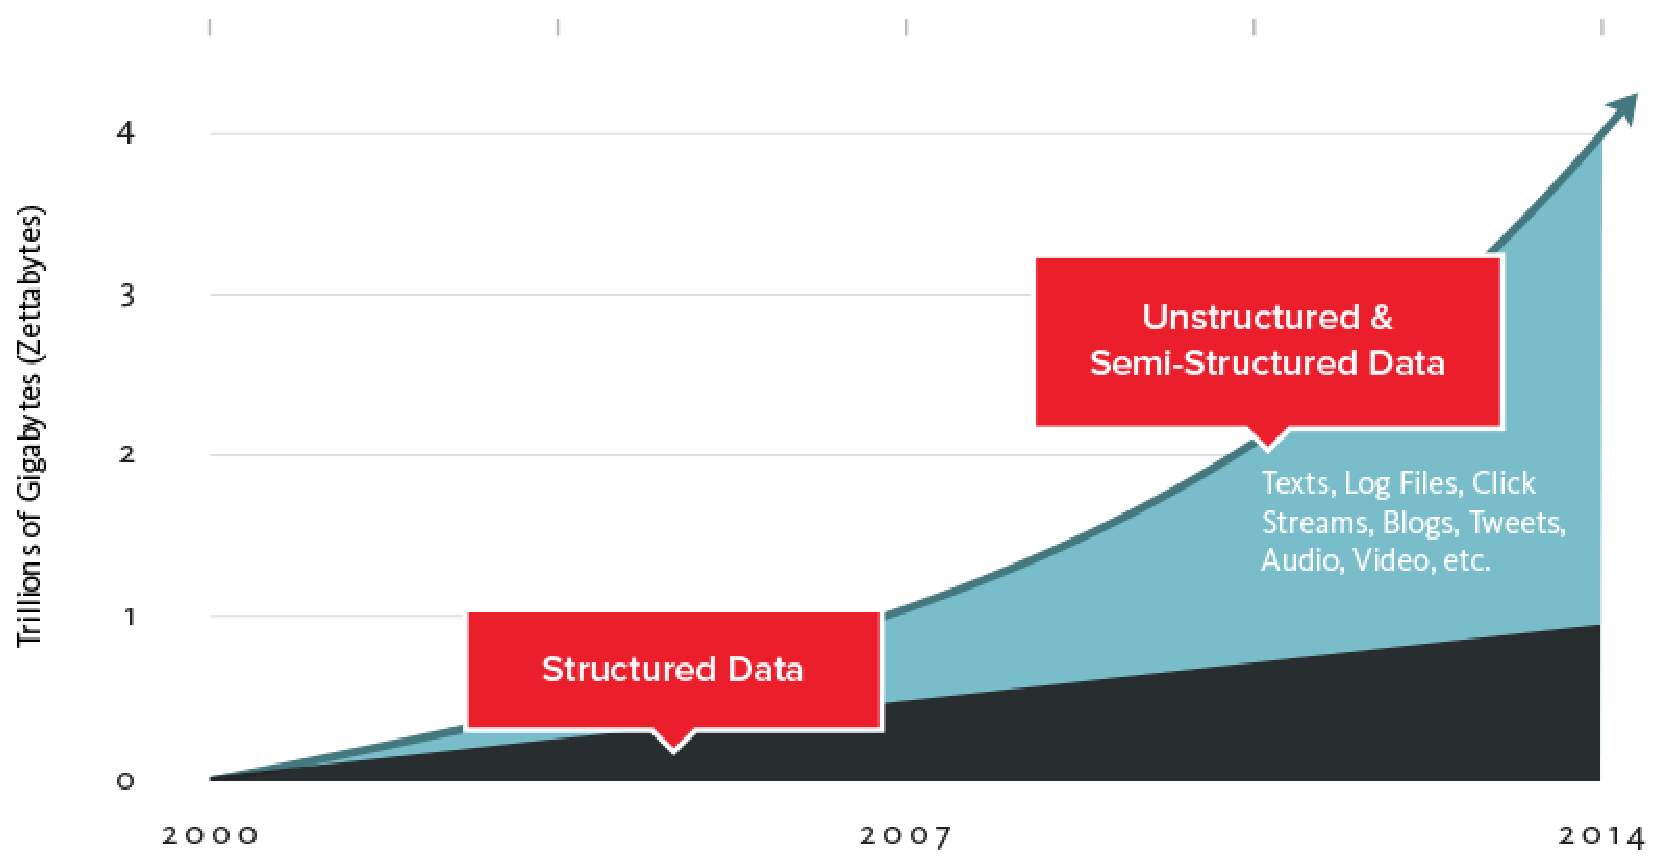
\includegraphics[width=10cm]{./img/why-nosql-2.eps}
		\caption{\tiny{Source: \url{http://www.couchbase.com/nosql-resources/what-is-no-sql}}}
	\end{figure}
\end{frame}

\begin{frame}
	\frametitle{How big are Big data?}
	\visible<2,3> {
		\begin{figure}
			\centering
			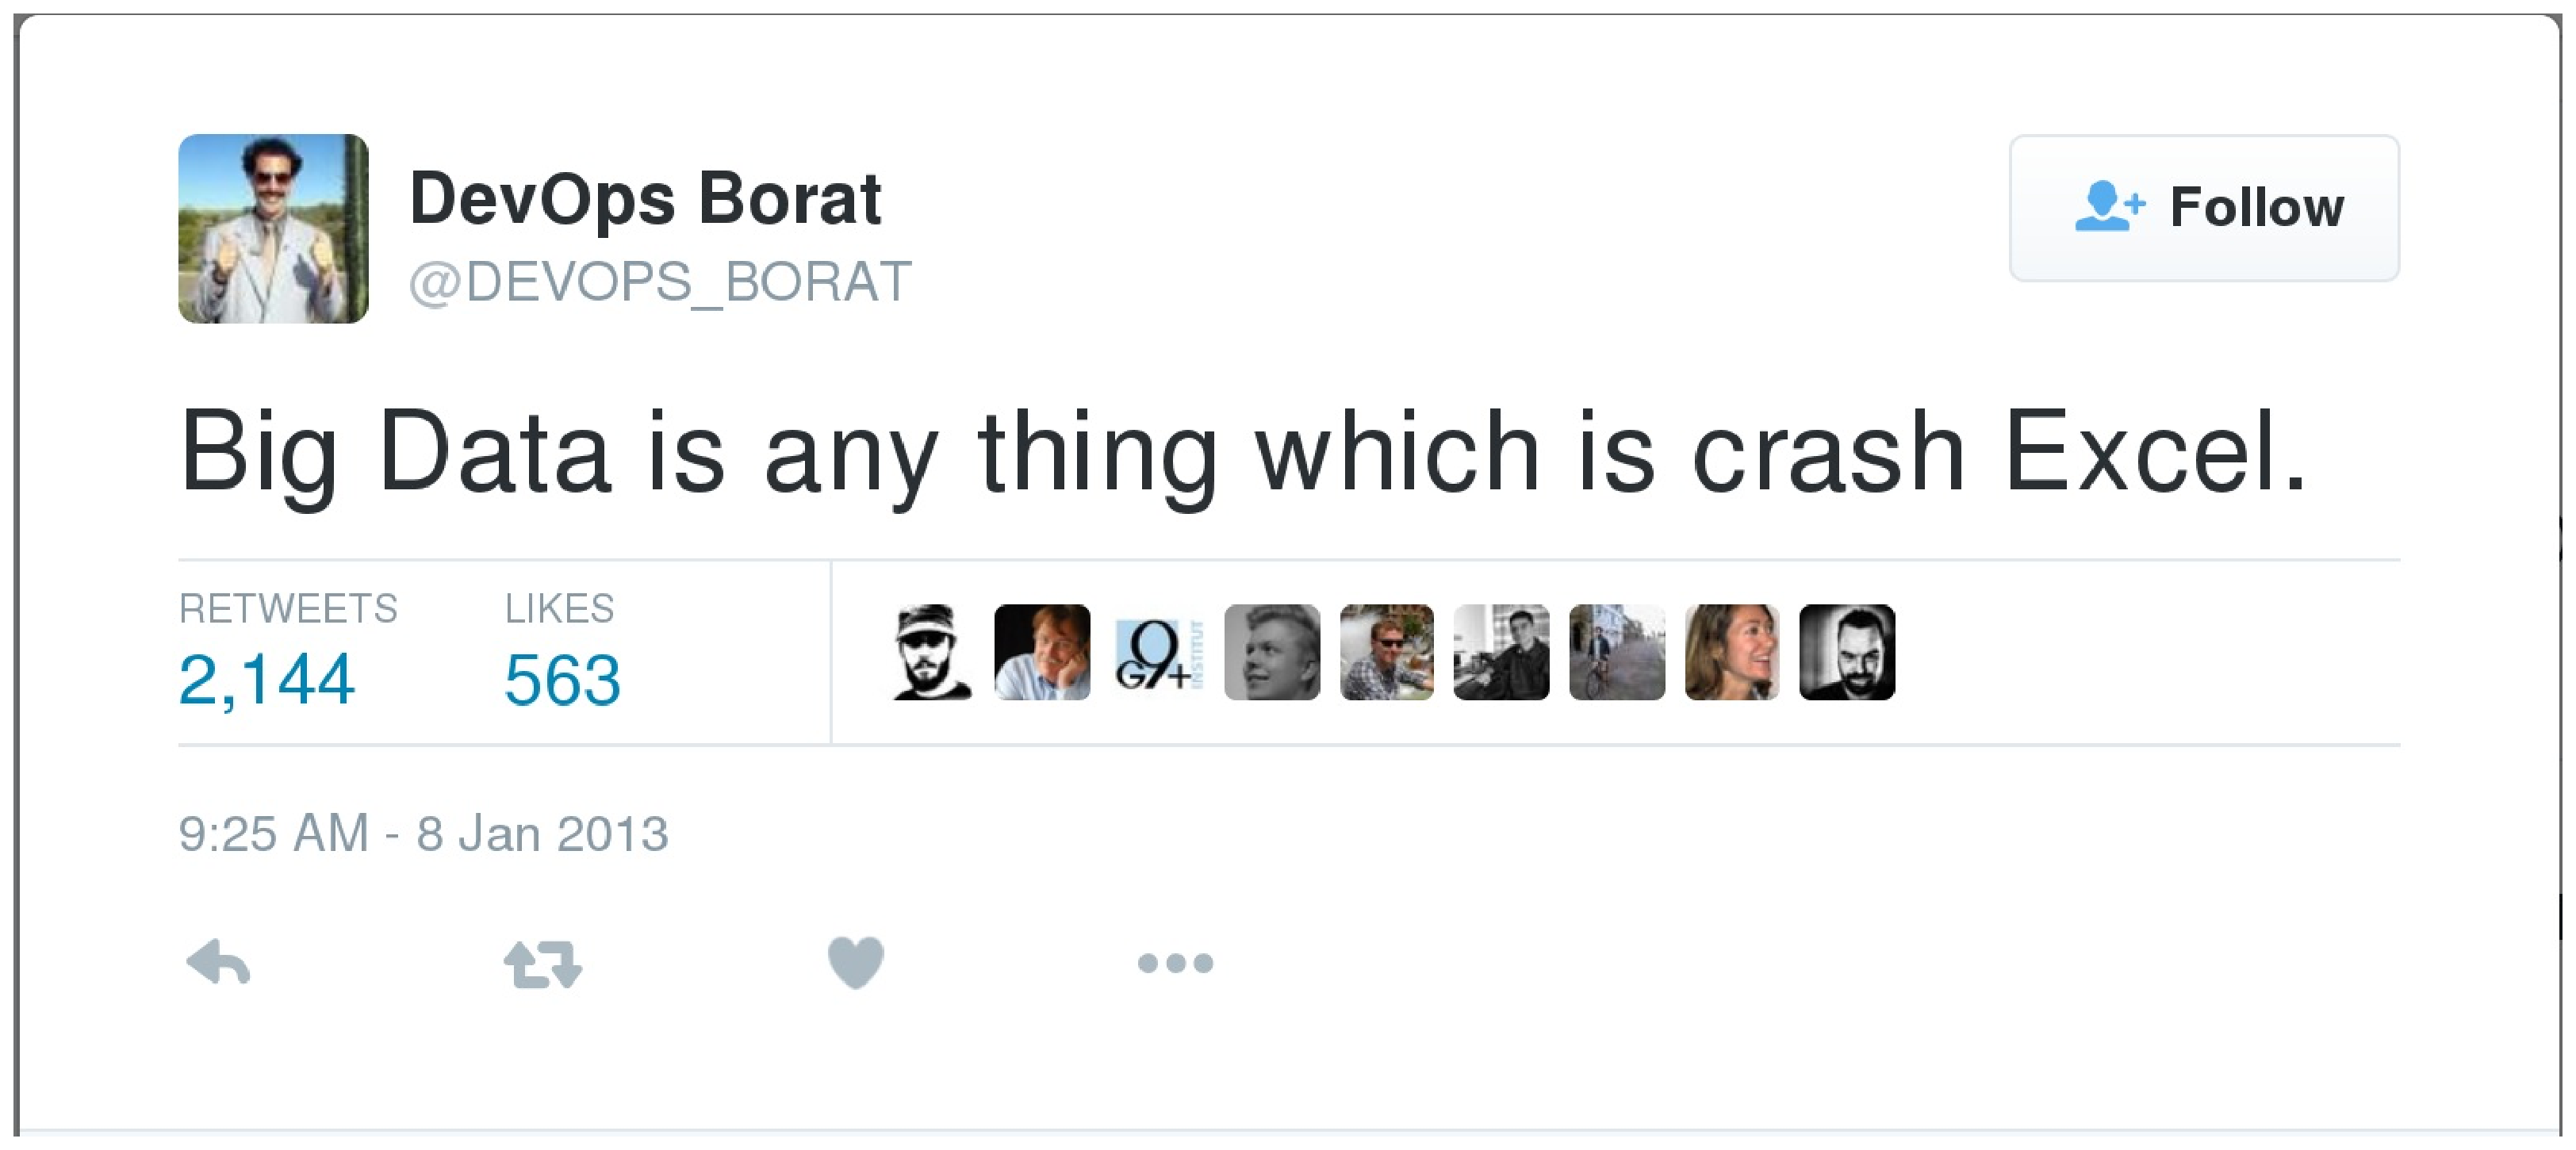
\includegraphics[width=8cm]{./img/borat_big_data.eps}
			\caption{\tiny{Source: \url{https://twitter.com/DEVOPS\_BORAT/status/288698056470315008}}}
		\end{figure}
	}
	\visible<3> {
		\begin{itemize}
			\item You can scale up, but sooner or later you'll probably have to scale out
			\item Need for highly scalable solution also because of cost effectiveness
		\end{itemize}
	}
\end{frame}

\begin{frame}
	\frametitle{Big data - challenges and approaches}
	\begin{itemize}
		\item Analysis run on top of the huge amount of data
		\item Ability to store huge amount of unstructured data (often for performance reasons)
		\item But also ability  to talk to RDBMS or query structured data is often needed as well
		\item Scalable solution
		\item Cloud architecture - everything is ephemeral
	\end{itemize}

	\visible<2,3> {	
		\vspace{0.5cm}
		\textbf{How these challenges are usually addressed:}
			\begin{itemize}
			\item Data replication
			\item Map-reduce model
		\end{itemize}
	}
	
	\visible<3> {
		\vspace{0.5cm}
		\textbf{Probably the most popular implementation:}
		\begin{itemize}
			\item
				\begin{figure}
					
\includegraphics[width=3cm, left]{./img/hadoop-logo.eps}
				\end{figure}	
		\end{itemize}
	}

\end{frame}

\begin{frame}
	\frametitle{Speeding up! I.}
	\vspace{0.5cm}
	\visible<1,2>{
		\centering{\textbf{\Large{Keep computation intensive data in memory}}} \\
	}
	\visible<2>{
		\vspace{1.5cm}
		\centering{\textbf{\Large{Don't replicate every single change of the data}}}
	}
\end{frame}

\begin{frame}
	\frametitle{Apache Spark}
	\begin{columns}
	\column{0.18\textwidth}
		\begin{figure}
			\centering
			
\includegraphics[width=2cm]{./img/spark-logo.eps}
		\end{figure}
	\column{0.8\textwidth}
	\textbf{Resilient Distributed Dataset (RDD)}
		\begin{itemize}
			\item Immutable distributed collection of data
			\item RDD is split into multiple partitions - can be located on different nodes
			\item Generated by a set of deterministic operations applied on a data source or other RDDs
			\item Provides 2 types of operations:
			\begin{itemize}
				\item \textbf{transformation} creates new RDD (e.g. \texttt{map()} or \texttt{filter()}) - return type is always RDD
				\item \textbf{action} computes a result from RDD (e.g. \texttt{count()} or \texttt{first()})
			\end{itemize}
			\item Lazy evaluation - only upon calling action on RDD
			\item RDD contains enough information (its linage) to be (re)created from a stable source 
			\item \color{blue}\href{https://www.usenix.org/conference/nsdi12/technical-sessions/presentation/zaharia}{M. Zaharia et al., NSDI, 2012}.
			% Rather than thinking of an RDD as containing specific data, it is best to think of each RDD as consisting of instructions on how to compute the data that we build up through transformations.
		\end{itemize}
	\end{columns}
\end{frame}
	
\begin{frame}
	\frametitle{Apache Spark}
		\begin{itemize}
			\item For some type of jobs (e.g. iterative algorithms) substantial speed up
			\item Speed up of one, sometimes even two orders of magnitude
		\end{itemize}
	  \begin{figure}
			\centering
			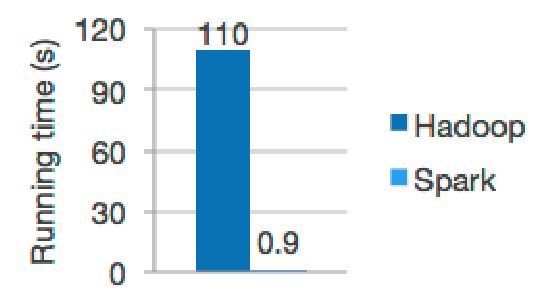
\includegraphics[width=6cm]{./img/hadoop_vs_spark.eps}
			\caption{\tiny{Logistic regression (an ML algorithm for classification) in Hadoop and Spark}}
			\vspace{-0.7cm}
			\caption{\tiny{Source: \url{http://spark.apache.org/}}}
		\end{figure}
\end{frame}

\begin{frame}
	\frametitle{Speeding up! II.}
	\vspace{0.5cm}
	\centering{\textbf{\Large{Process data immediately once it arrive}}}
	\vspace{0.5cm}
\end{frame}

\begin{frame}[fragile]
	\frametitle{Spark streaming}
	\begin{itemize}
	 \item Discretized Streams (DStreams) - RDD micro-batches
	 \item User defined (time) size of the batch
	\end{itemize}

	\begin{lstlisting}[style=Java]
		|val| conf = new SparkConf().setAppName("WordCount")
		|val| ssc = new StreamingContext(conf, `Seconds(1)`)
	\end{lstlisting}
	
	\begin{figure}
		\centering
		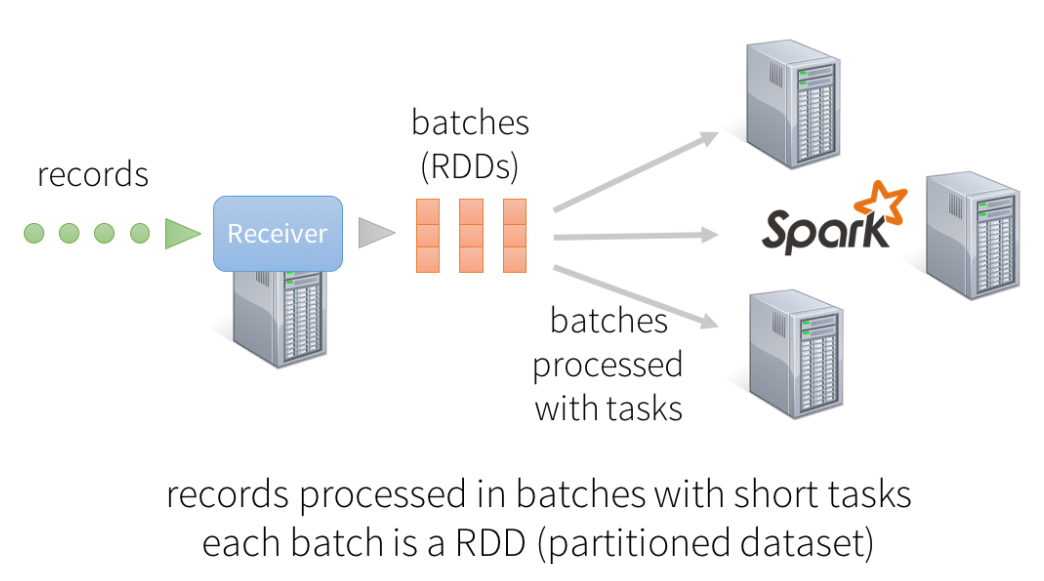
\includegraphics[width=7cm]{./img/spark-streaming2.eps}
		\caption{\tiny{Source: \url{https://databricks.com/blog/2015/07/30/diving-into-spark-streamings-execution-model.html}}}
	\end{figure}
\end{frame}

\begin{frame}[fragile]
	\frametitle{Spark streaming}
	\begin{lstlisting}[style=Java]
    // Split each line into words
    |val| words = lines.flatMap(_.split(" "))
	\end{lstlisting}

	\begin{figure}
		\centering
		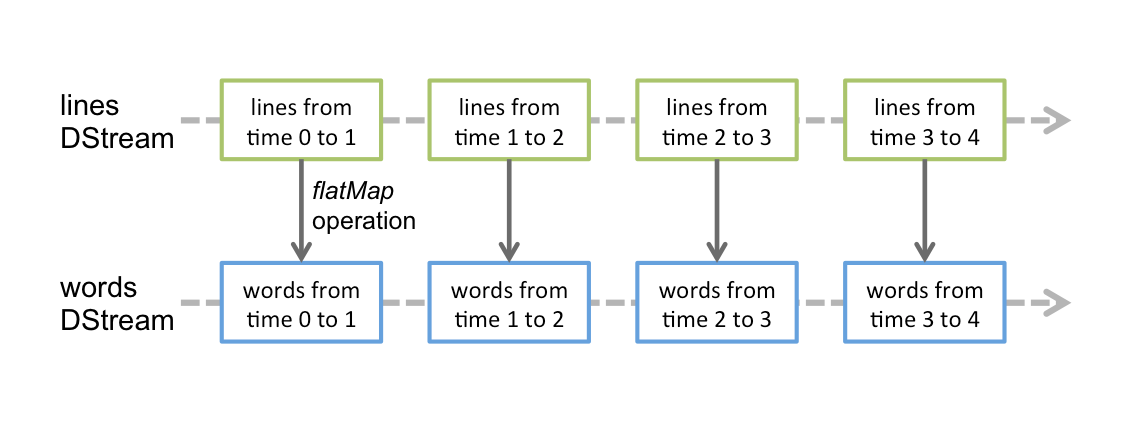
\includegraphics[width=12cm]{./img/streaming-dstream-ops.eps}
		\caption{\tiny{Source: \url{http://spark.apache.org/docs/latest/streaming-programming-guide.html}}}
	\end{figure}
\end{frame}


\begin{frame}
	\frametitle{Homework for you: Real-time stream processing frameworks}
	\begin{columns}
	\column{0.45\textwidth}
		\begin{figure}
			\centering
			
\includegraphics[width=3cm]{./img/storm-logo.eps}
		\end{figure}
	\column{0.55\textwidth}
		\vspace{-0.5cm}
		\textbf{\Large{Apache Storm}} 
	\end{columns}

	\vspace{1cm}
	
	\begin{columns}
	\column{0.45\textwidth}
		\begin{figure}
			\centering
			
\includegraphics[width=1.5cm]{./img/flink-logo.eps}
		\end{figure}
	\column{0.55\textwidth}
		\vspace{-0.5cm}
		\textbf{\Large{Apache Flink}}
	\end{columns}
	
	\vspace{1cm}
	
	\begin{columns}
	\column{0.45\textwidth}
		\begin{figure}
			\centering
			
\includegraphics[width=3cm]{./img/samza.eps}
		\end{figure}
	\column{0.55\textwidth}
		\vspace{-0.5cm}
		\textbf{\Large{Apache Samza}}
	\end{columns}
\end{frame}

\begin{frame}
	\frametitle{Speeding up! III.}
	
	\vspace{0.5cm}
	\centering{\textbf{\Large{Keep the data in memory all the time}}}
	\vspace{0.5cm}
	
	\begin{figure}
		\centering
		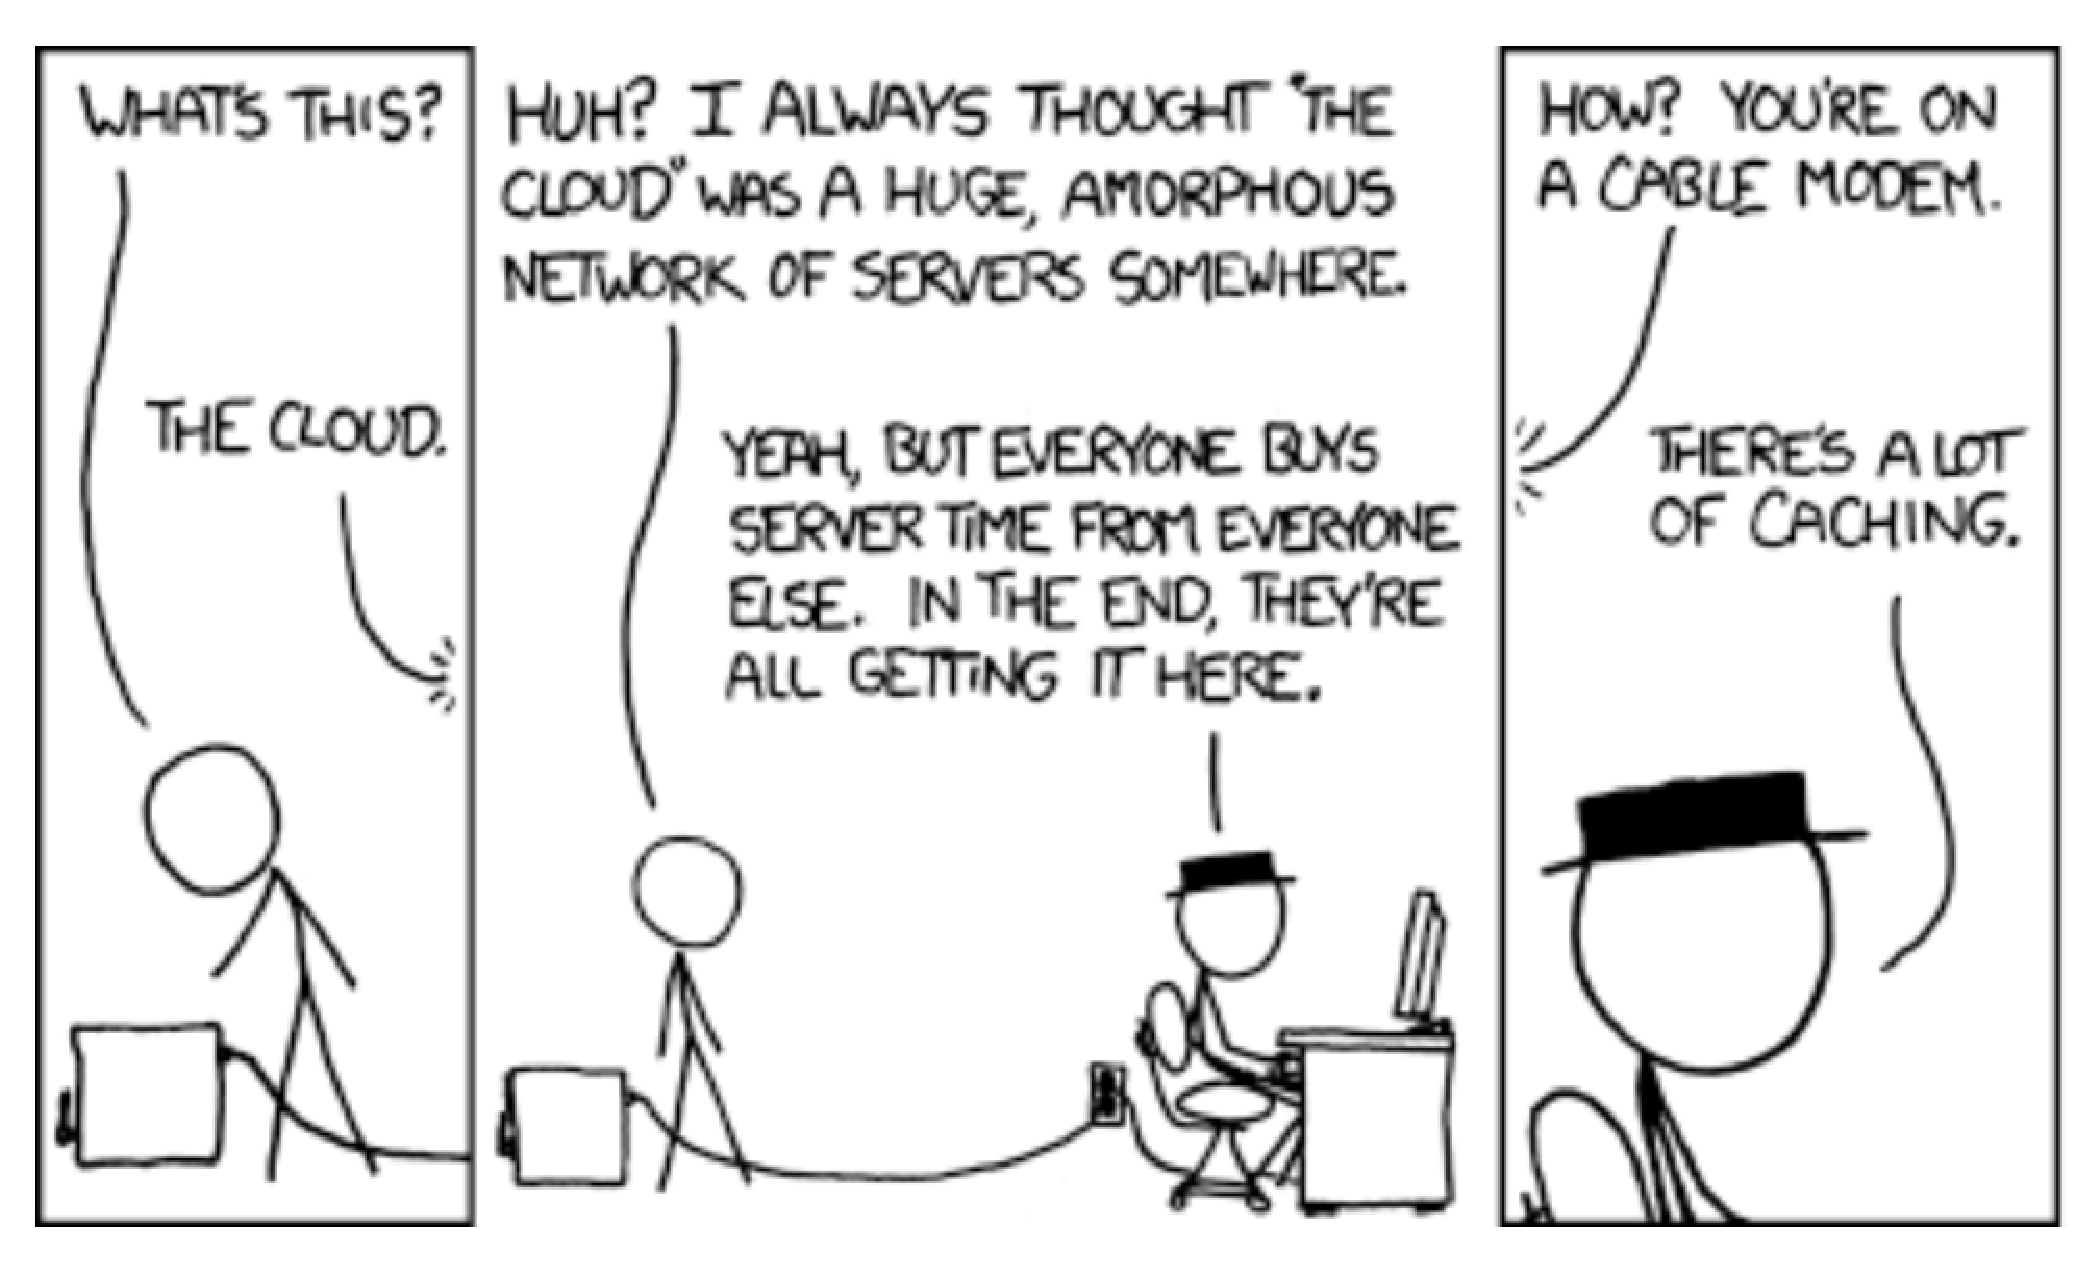
\includegraphics[width=8cm]{./img/xkcd_908.eps}
		\caption{\tiny{Source: Part of \href{http://xkcd.com/908/}{xkcd \#908}}}
	\end{figure}
\end{frame}

\begin{frame}
	\frametitle{In-memory data grid: Infinispan}
	\begin{columns}
	\column{0.38\textwidth}
		\begin{figure}
			\centering
			
\includegraphics[width=3cm]{./img/infinispan.eps}
		\end{figure}
	\column{0.6\textwidth}
		\begin{itemize}
			\item Data grid platform, written in Java
			\item In-memory No-SQL key-value data store, (optionally) schema-less
			\item Distributed cache - offers massive memory
			\item Elastic and scalable - can run on hundreds of nodes
			\item Highly available - no SPOF, resilient to node failures
			\item Transactional
			\item Supports indexing and searching
			\item Many other features
		\end{itemize}
	\end{columns}
\end{frame}

\begin{frame}[fragile]
	\frametitle{Infinispan integration with Spark}
	\begin{itemize}
		\item Spark partitions contain only cache segments owned by the associated ISPN server
		\item Connector enables read ISPN data from Spark or write Spark data to ISPN
	\end{itemize}
	\vspace{0.3cm}
%	\visible<1,2> {
	Creating RDD from data in ISPN cache
	\begin{lstlisting}[style=Java]
    |val| config = new Properties
    config.put("infinispan.rdd.cacheName", "my-cache")
    config.put("infinispan.client.hotrod.server_list", "127.0.0.1:11222")
    |val| ispnStream = new InfinispanInputDStream[String, Double](ssc, `StorageLevel.MEMORY_ONLY`, config) //for String Double pairs
	\end{lstlisting}
%  }
	\vspace{0.3cm}
%	\visible<2> {
	Creating DStream from data in ISPN cache
	\begin{lstlisting}[style=Java]
    //same config as in previous example
    |val| ispnStream = new InfinispanInputDStream[String, Double](ssc, `StorageLevel.MEMORY_ONLY`, config)
	\end{lstlisting}
%  }
\end{frame}

\begin{frame}[fragile]
	\frametitle{Infinispan integration with Spark}
	\begin{itemize}
	 \item ISPN server side filters and converters can be used for adjusting RDDs when created 
	 \item ISPN queries can be applied to RDDs
	\end{itemize}
	\vspace{0.5cm}
%	\visible<1,2> {
	Creating RDD/DStream by querying ISPN cache
	\begin{lstlisting}[style=Java]
    |val| query = Search.getQueryFactory(cache).from(classOf[User]).having("name").equal("Vojtech").toBuilder[RemoteQuery].build
    |val| filteredRDD = rdd.filterByQuery(query, classOf[User])
	\end{lstlisting}
%	}
	\vspace{0.5cm}
%	\visible<2> {
	Writing RDD/DStream to ISPN cache
		\begin{lstlisting}[style=Java]
    //same config as in previous examples
    InfinispanDStream[String, Double](temperatureStream).writeToInfinispan(config)
	\end{lstlisting}
%	}
\end{frame}

\begin{frame}[fragile]
	\frametitle{Few other ISPN highlights wrt. fast data processing}
	\begin{itemize}
	 \item Event listeners
	\end{itemize}
	\begin{lstlisting}[style=Java,basicstyle=\tiny\ttfamily]
    `@ClientListener`
    public static class MyListener {
        `@ClientCacheEntryCreated`
        `@ClientCacheEntryModified`
        public void onEntryChange(ClientCacheEntryModifiedEvent<String> event) {
           //TODO some action when entry is created or modified
        }

        `@ClientCacheEntryRemoved`
        `@ClientCacheEntryExpired`
        public void entryRemove(ClientCacheEntryRemovedEvent<String> event) {
          //TODO some action when entry is removed or expired
        }
    }
	\end{lstlisting}
	
	\begin{itemize}
	 \item Continuous query
	\end{itemize}
	\begin{lstlisting}[style=Java,basicstyle=\tiny\ttfamily]
    QueryFactory qf = Search.getQueryFactory(myCache);
    Query query = qf.from(User.class).select("name").having("age").lte(30).toBuilder().build();
    `ContinuousQueryListener<Object, Object> listener = new MyListenerI<Object, Object>();
    ContinuousQuery<Object, Object> cq = new ContinuousQuery<>(cache);
    cq.addContinuousQueryListener(listener, query);`
	\end{lstlisting}
	
	\begin{itemize}
			\item Distributed streams - implementation of \texttt{java.util.stream.Stream} over (distributed!) cache data
		\end{itemize}
\end{frame}

\begin{frame}
	\frametitle{Where do we get from Big data?}
	\visible<1,2,3,4,5>{
	\begin{itemize}
		\pause
		\item Data is kept in memory all the time and thus processing and exchanging the data is much faster
		\pause
		\item Data is processed once it arrives
		\pause
		\item Results of the analysis can be pushed to user by various means, e.g. using continuous queries
	\end{itemize}
	}
	\vspace{0.5cm}
	\visible<5>{
		\centering{\textbf{\LARGE{== Fast data?}}}
	}
\end{frame}

\begin{frame}
	\frametitle{"Hello world" Demo}
	\centering
	\textbf{Infinispan integration with Apache Spark:} \\
	\vspace{1cm}
	\textbf{Temperature average}
	\begin{itemize}
	 \item Stream of temperature measurements from different places stored into Infinispan
	 \item Average temperature is continually recomputed for each place in Spark
	 \item Results are stored back in Infinispan
	\end{itemize}
	\vspace{1cm}
	Sources available on \textbf{\scriptsize{\color{blue}{\url{https://github.com/vjuranek/presentations/tree/master/DevConf_Brno2016}}}}
\end{frame}

\begin{frame}
	\frametitle{"Hello world" Demo}
	\visible<1,2,3,4,5>{
	\begin{figure}
		\centering
		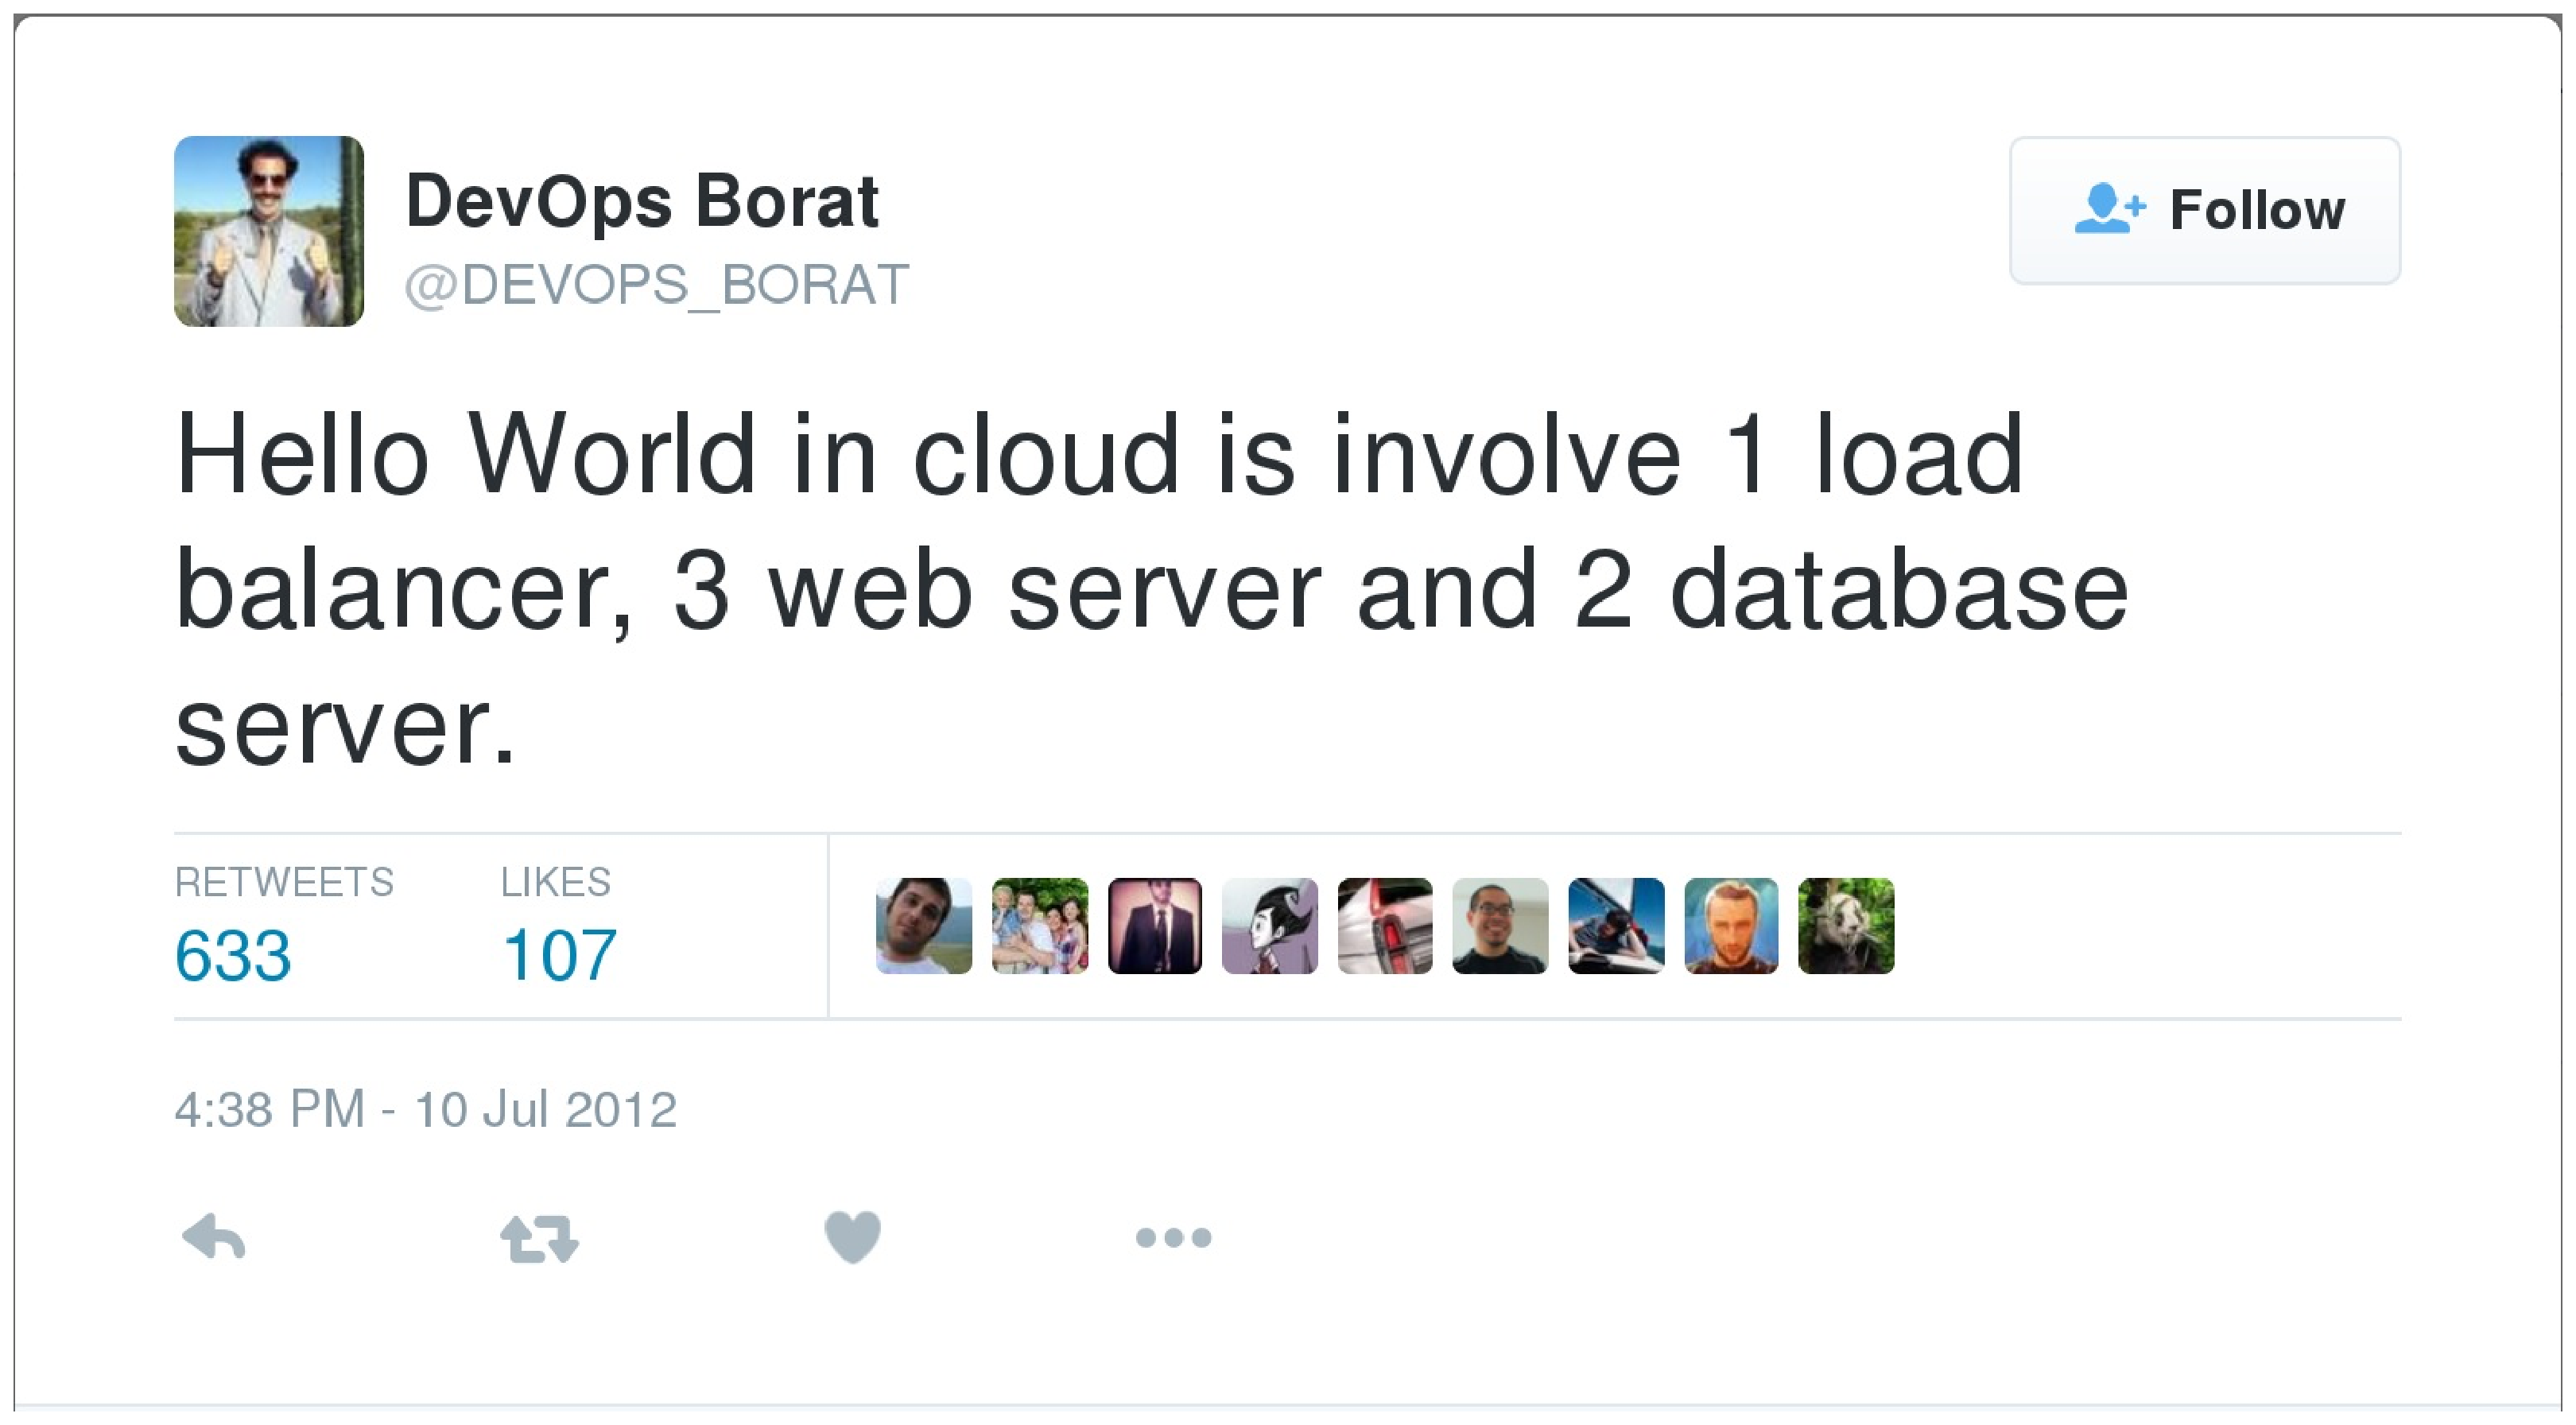
\includegraphics[width=7cm]{./img/borat_hello_world.eps}
		\vspace{-0.3cm}
		\caption{\tiny{Source: \url{https://twitter.com/DEVOPS\_BORAT/status/222837225921060864}}}
	\end{figure}
	}
	\vspace{-0.2cm}
	\visible<2,3,4,5>{
	\begin{itemize}
		\pause
		\item One Infinispan server for storing incoming data and results
		\pause
		\item One app randomly generating place and temperature (simulating e.g. network of temperature sensors)
		\pause
		\item Spark streaming for analyzing the data 
		\pause
		\item Client app showing result data when they arrive, using Infinispan cache listener
	\end{itemize}
	}
\end{frame}

\begin{frame}
	\frametitle{Summary}
	\vspace{3cm}
	\centering{\textbf{\LARGE{Do the data analysis with frameworks which keep the data in memory during processing}}}
	\vspace{3cm}
\end{frame}

\begin{frame}
	\frametitle{Summary}
	\vspace{3cm}
	\centering{\textbf{\LARGE{Process data once it arrives}}}
	\vspace{3cm}
\end{frame}

\begin{frame}
	\frametitle{Summary}
	\vspace{3cm}
	\centering{\textbf{\LARGE{If possible, keep data in memory during whole application stack}}}
	\vspace{3cm}
\end{frame}

\begin{frame}
	\frametitle{Summary}
	\vspace{3cm}
	\centering{\textbf{\LARGE{Infinispan provides many useful features like integration with Apache Spark, continuous query, cache listeners and many others}}}
	\vspace{3cm}
\end{frame}


\begin{frame}
	\frametitle{Summary}
	\begin{itemize}
		\item Do the data analysis with frameworks which keep the data in memory during processing
		\item Process data once it arrives
		\item If possible, keep data in memory during whole application stack
		\item Infinispan provides many useful features like integration with Apache Spark, continuous query, cache listeners and many others
	\end{itemize}
\end{frame}


\begin{frame}
	\frametitle{Question?}
	\begin{figure}
		\centering
		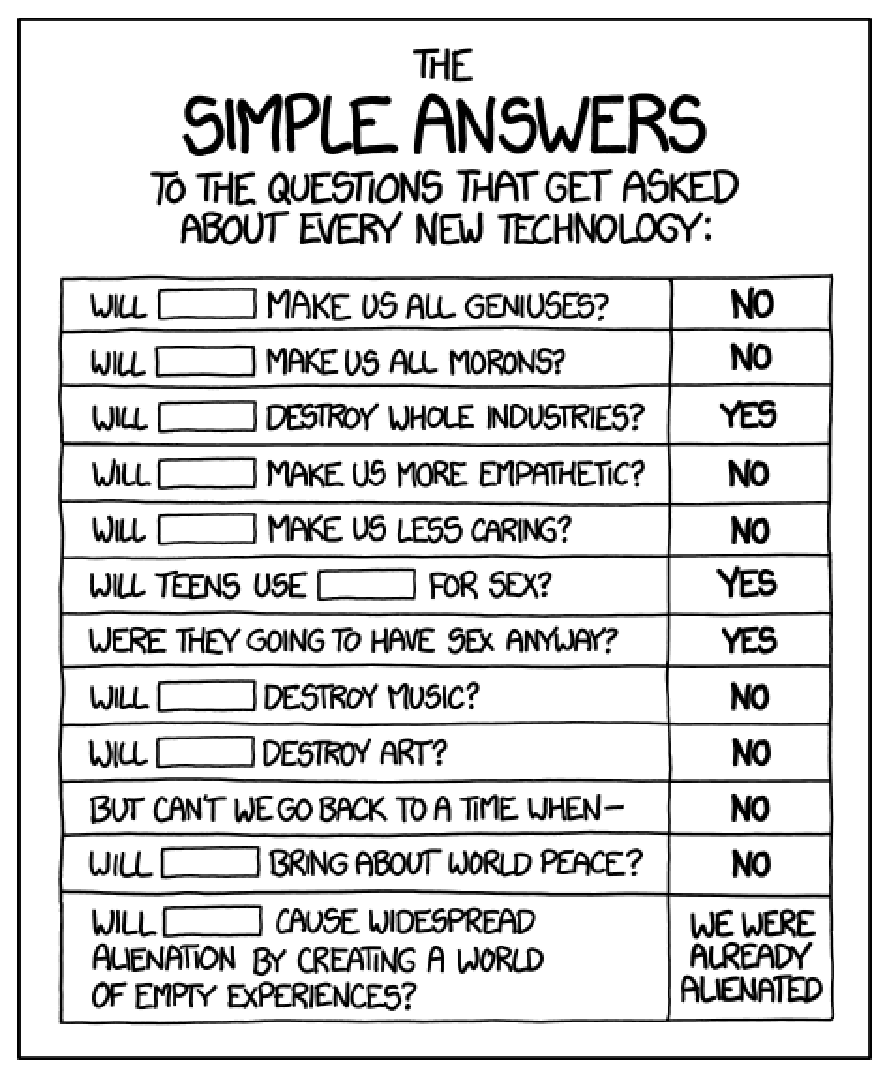
\includegraphics[width=6cm]{./img/simple_answers.eps}
		\caption{\tiny{Source: \url{https://xkcd.com/1289/}}}
	\end{figure}
\end{frame}

\begin{frame}
	\begin{figure}
		\centering
		
\includegraphics[width=2.5cm]{./img/infinispan8.eps}
	\end{figure}
	\centering
	\large{\color{blue}{\url{http://infinispan.org/}}} \\
	\vspace{1cm}
	\huge{\textbf{Thank you for your attention!}} \\
	%\vspace{1cm}
	%\huge{\textbf{Questions?}}
\end{frame}

\end{document}